\section{Text Analysis}
\subsection{Text Data Access}
L'obiettivo principale del text data access è di connettere user con le giuste informazioni al momento giusto. Questa operazione può essere svolta in due modi: \begin{itemize}
    \item pull, dove l'user prende l'iniziativa di cercare le info ed estrapolarle dal sistema
    \item push, dove il sistema prende l'iniziativa e offre informazioni all'user. 
\end{itemize}
Ci sono due modi per interrogare una collezione di dati, il \textit{search engine} e \textit{sistema di raccomandazione}. Nel primo caso siamo noi a dare la query. Nell'altro caso, è tipo su netflix che consiglia delle serie. Quindi pull è il search engine, push è raccomandazione. Prende il nome di \textit{Text retrieval} quello che noi abbiamo appena descritto come search engine, ovvero trovare un informazione tramite query. 
\\
Problema solitamente complesso: non è una semplice query in un database che fornisce un risultato esatto. La risposta desiderata è anche soggettiva, dipende dalla correttezza della query scritta dall'utente (basta pensare alla ricerca su Google e come cambiano i risultati sulla base di ciò che si cerca). 

\subsection{Text Retrieval}
Data una collezione di documenti, il text retrieval può essere definito come: utilizzando una query dell'user, (per esempio, una \textit{descrizione} dell'informazione ricercata) identificare un subset di documenti che soddisfano la richiesta. 
\begin{itemize}
    \item Abbiamo V vocabolario di tutte le parole di un natural language.
    \item q, query dell'user, dove $q_i$ $\in$ V
    \item $d_i$, documento tale che $d_{ij}$ $\in$ V
    \item la query è più corta del documento
    \item una collezione C è l'insieme di documenti d
    \item assumiamo che esista un sottoinsieme R di documenti, che sono rilevanti per la query q
\end{itemize}
Il sottoinsieme perfetto R(q) non è sempre il risultato. Per correttezza, considereremo un R'(q), come un'approssimazione del risultato esatto R(q) comunque accettabile. 
\\
\textbf{Come possiamo trovare quindi R'(q)?} Esistono due metodi: \textit{document selection} o \textit{document ranking}.

\subsubsection{Document Selection vs Document Ranking}
La document selection utilizza un classificatore binario per classificare se un documento è relevant o no rispettando una particolare query. Usando questa strategia, il sistema capisce l'effettiva rilevanza di un documento. 
\\
Nel document ranking, abbiamo una funzione di ranking e l'user sceglie un limite. In questo caso, il sistema impara una rilevanza relativa: quali documenti potrebbero essere rilevanti. Per il principio del probability ranking, fare un ranking decrescente di rilevanza fornisce una informazione utile se l'utilità di un documento per l'user è indipendente dall'utilità degli altri documenti e se l'user potrà guardare la lista dei risultati sequenzialmente.

\subsection{Retrieval Models}
Esistono diversi modelli per fare retrieval, e si distinguono per tipologia di approccio al problema. Alcuni sono basati sempre sul concetto di similarità, altri lavorano sul piano probabilistico. Molti modelli si basano anche sulla consapevolezza che i documenti di testo vengono rappresentati come bag of words, non shingles. Si sceglie un vocabolario (lingua) di riferimento e si usa quello.
\\
\begin{figure}[th]
    \centering
    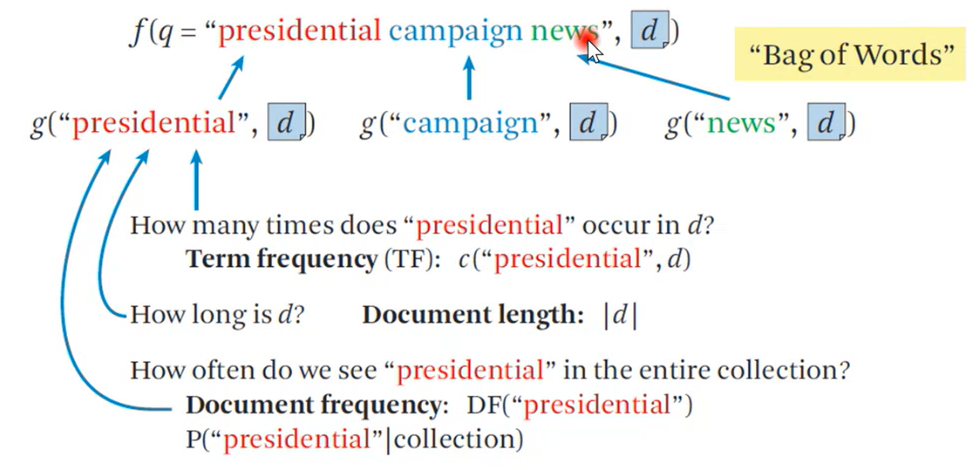
\includegraphics[scale=0.5]{Text Analysis/img/bagofwords.png}
\end{figure}
\\
Ma allora come faccio a decidere quale documento è più importante? Per esempio posso contare le occorrenze della parola ricercata, oppure tenere conto quanto è lungo il documento, poichè più parole ci sono, più è probabile che almeno una delle parole della mia query compaia nella ricerca; un ultimo valore che è necessario conoscere sono le stop words: parole "inutili". Quando, quanto ecc... sono parole che non ci interessano quindi le eliminiamo. Poi ci sono parole importanti, che dipendono dal dominio della ricerca. In un documento di calcio, "Goal" è una parola molto frequente, meno discriminatoria nella ricerca. Ma una parola come "Messi", è molto più specifica. Questo effetto prende il nome di document frequency (spiegato meglio in seguito). 
\\
Le metriche più importanti sono sicuramente \textbf{term frequency} e \textbf{document frequency} quando si parla della funzione di ranking (che chiameremo TF e DF).

\subsubsection{Vector Space Retrieval Model}
Modello molto semplice basato sulla similarità che trasforma i documenti della collezione in vettori e anche la query dell'utente. 
\\
\begin{figure}[th]
    \centering
    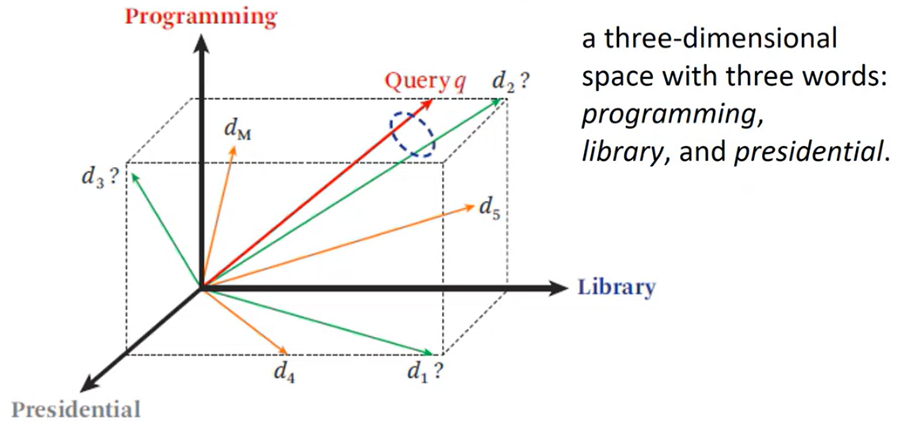
\includegraphics[scale=0.5]{Text Analysis/img/vector space retrieval.png}
\end{figure}
\\
Vado ad orientarli nello spazio e guardo quelli che sono più vicini al vettore della query. Per esempio nell'immagine parliamo di d2. 
\\
\textbf{Come trasformiamo una query in un vettore?} Stabilisco un vocabolario, di parole, ogni parola è una componente e ha una misura che dipende dalle occorrenze della parola. Dopo è necessario calcolare la distanza: coseno dell'angolo sotteso tra i due vettori. Più i vettori sono allineati, più l'angolo tende a 0, più il coseno tende a 1, \textit{più i vettori sono simili}. 
\\
Vediamo ora le tecniche per la ricerca di similarità utilizzando questo modello:
\begin{itemize}
    \item Vector Space Model Booleano: mi rappresenta le parole con 1 se è presente, 0 se non è presente. Utilizziamo poi il dot product per trovare la similarità: Sim(q,d) = q.d = $\sum_{i=1}^{N} x_i y_i$ dove le x sono in q, e le y sono in d. Non funziona quasi mai purtroppo, perchè è troppo semplice non considera il TF.
    \item Improved VSM Instantiation: miglioriamo la tecnica precedente aggiungendo TF. Non consideriamo più l'i-esimo elemento di q e d come 1 o 0 in base alla presenza della parola ma lo sostituiamo con il numero di volte che essa compare.  
    \item IDF Approach: non basta nemmeno aggiungere TF, allora mettiamo anche IDF che è l'inverso della DF. Utilizziamo la IDF perchè la DF sarebbe il numero di elementi in cui una certa parola appare, ma vogliamo penalizzare le parole che appaiono in troppi documenti, quindi usiamo il suo inverso. 
    \begin{center}
        \begin{math}
            IDF(w) = \frac{M+1}{DF(w)}
        \end{math}
    \end{center}
    E usiamo il suo logaritmo per smorzare alcuni valori troppo elevati. Ottenuto tale valore comunque, sfruttiamo TF come prima ma ci moltiplichiamo IDF che funge da peso. 
    \begin{center}
        \begin{math}
            f(q,d) = \sum_{i=1}^{N} x_i y_i = \sum c(w, q) c(w, d) log(\frac{M+1}{DF(w)})
        \end{math}
    \end{center}
    \item TF Transformation: l'approccio descritto nel punto precedente ha comunque un problema, la probabilità varia linearmente all'aumentare di TF; per esempio basta che la parola "cipolla" sia presente 2 volte che quel documento ottiene una probabilità doppia rispetto ad un documento dove appare una sola volta. Per compensare andiamo a smorzare TF ad esempio mettendo 1+log(1+TF).
    \item State-of-Art VSM Ranking Functions: pivoted lenght e BM25 si basano su altri parametri aggiunti che modificano il TF. BM25 sfrutta questa formula: 
    \begin{center}
        \begin{math}
            y = \frac{(k+1)TF}{TF+k}
        \end{math}
    \end{center}
    Dove k+1 è il valore massimo che il TF può raggiungere. Se non è presente la parola, vale 0, altrimenti tenderà a k+1. Pivoted lenght si basa invece sulla lunghezza del documento. 
\end{itemize}

\newpage    

\subsection{Probabilistic Retrieval Models}
Determinare, dato il documento e data la query, quanto esso sia rilevante. Si vede bene in questo esempio:
\\
\begin{figure}[th]
    \centering
    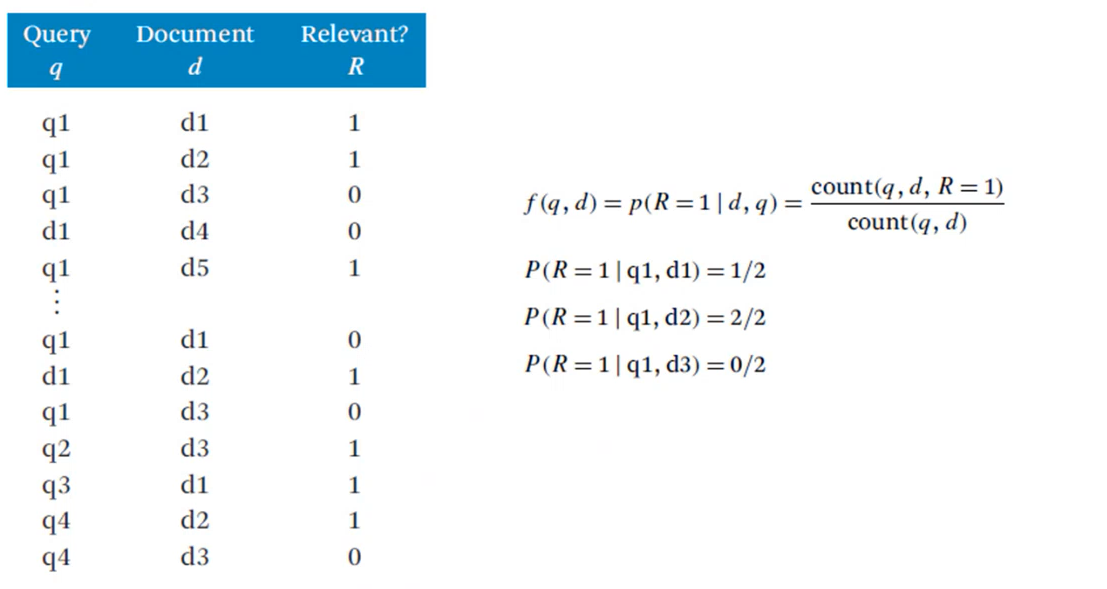
\includegraphics[scale=0.5]{Text Analysis/img/example.png}
\end{figure}
\\
Confronta più risposte sulla domanda di rilevanza, come se confrontassi la risposta di più utenti. Approssimiamo la rilevanza alla probabilità:
\begin{center}
    \begin{math}
        p(R=1|d,q) = p(q|d,R=1)
    \end{math}
\end{center}
Della query, data una rilevanza e un documento. Quindi la domanda diventa:
\begin{center}
    \textit{Qual è la query che mi dà come risultato tale documento?}
\end{center}
Perchè è vantaggioso? Posso stimare le query ipotetiche, senza averne necessariamente una. 

\subsubsection{Text statistics: Zipf's Law}
Il rank di una parola moltiplicato per la frequenza di tale parola è una costante.
\begin{center}
    \begin{math}
        r \times f = k
    \end{math}
\end{center}
Quello che dice questa legge, nello specifico, è che ci saranno poche parole che appaiono tantissimo (le parole più frequenti) ma si decresce in maniera non lineare, quindi ci saranno tantissime parole che appaiono pochissimo. 

\subsubsection{Language Model}
Il language model è una probabilità che io assegno ad una frase. Si suddivide in:
\begin{itemize}
    \item machine translation: traduzione linguistica corretta
    \item correzione di pronuncia 
    \item speech recognition: p(I saw a van) $>>$ p(eyes awe of an)
\end{itemize}
E tanti altri. Nel probabilistic language modeling l'obiettivo è quello di calcolare la probabilità di una frase o sequenza di parole. In questo modo, un'altra task correlata è sicuramente la prediction della upcoming word. 
\\
A livello matematico, l'obiettivo è quello di calcolare la probabilità di una parola w data una history h = $p(w|h)$; per farlo ci possiamo affidare alla \textit{chain rule of probability}, cerchiamo di suddividere il problema, dove la probabilità di una frase diventa:
\begin{center}
    \begin{math}
        P(A,B,C,D) = P(A)P(B|A)P(C|A,B)P(D|A,B,C)
    \end{math}
\end{center}
Ma non arriviamo ad un grande risultato perchè con frasi troppo lunghe sono troppo complesse. Dobbiamo usare dei bigrammi! Usiamo solo l'elemento precedente. Quindi in un documento invece di andare a visualizzare intere frasi, guardiamo solo la parola che precede. Il calcolo della probabilità, in quel caso, diventa: 
\begin{center}
    \begin{math}
        P(w_i | w_{i-1}) = \frac{count(w_{i-1}w_i)}{\sum count(w_{i-1}w)}
    \end{math}
\end{center}
Ovvero la probabilità della coppia che sto esaminando, diviso il numero di correlazioni tra la parola precedente e un'altra qualsiasi parola che non sia quella giusta. Il discorso è comunque analogo nel caso di trigrammi, o nel caso considerassimo k parole alla volta con k $>$ 3. 
\\
\textbf{Come è cambiata con il machine learning?} Non è capace, un modello machine learning non riesce con troppi dati, ma una rete neurale sì. 
\\
Ovviamente vado poi a moltiplicare (come mostrato in alto) la probabilità di ogni bigramma fino ad ottenere la probabilità di una frase. 
\\
\begin{figure}[th]
    \centering
    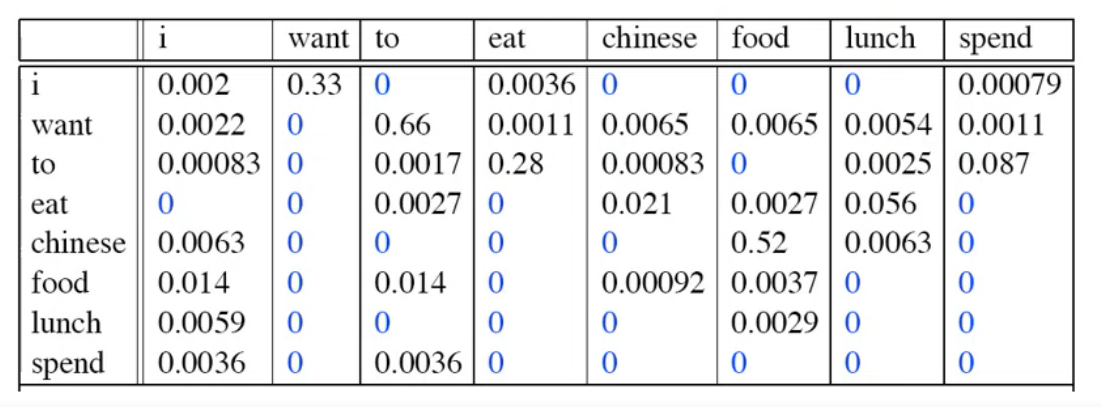
\includegraphics[scale=0.45]{Text Analysis/img/bigrams.png}
\end{figure}
\\
In questa immagine è possibile visualizzare un esempio di calcolo su bigrammi. Una domanda sorge spontanea, come vengono gestiti gli 0? Potrebbero dare problemi di generalizzazione! Allora per evitare che ci sia uno 0, possiamo utilizzare la tecnica di Laplace Smoothing, per cui aggiungiamo un 1 al conteggio di tutto. 
\\
\begin{figure}[th]
    \centering
    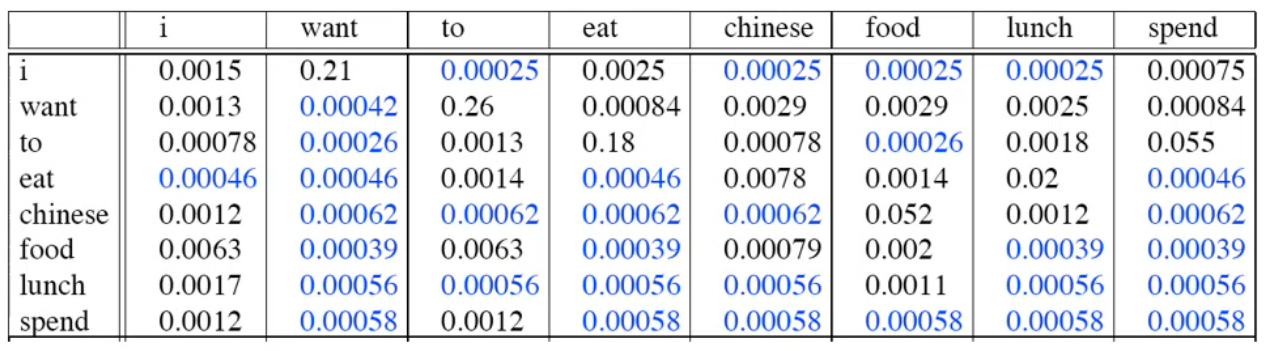
\includegraphics[scale=0.45]{Text Analysis/img/laplacesmoothing.png}
\end{figure}
\\
I risultati della tabella cambiano di tanto! E non solo gli zeri.

\newpage

Quello che avviene infatti nel Laplace Smoothing non è solo un aumento di 1 del conteggio, ma quando vado a calcolare le probabilità:
\begin{center}
    \begin{math}
        P(w_i | w_{i-1}) = \frac{count(w_{i-1}w_i) + 1}{\sum count(w_{i-1}w) + V}
    \end{math}
\end{center}
Al denominatore vado anche a mettere il vocabolario V. Quindi il conteggio nelle tabelle, prima e dopo Laplace, cambia: 
\\
\begin{figure}[th]
    \centering
    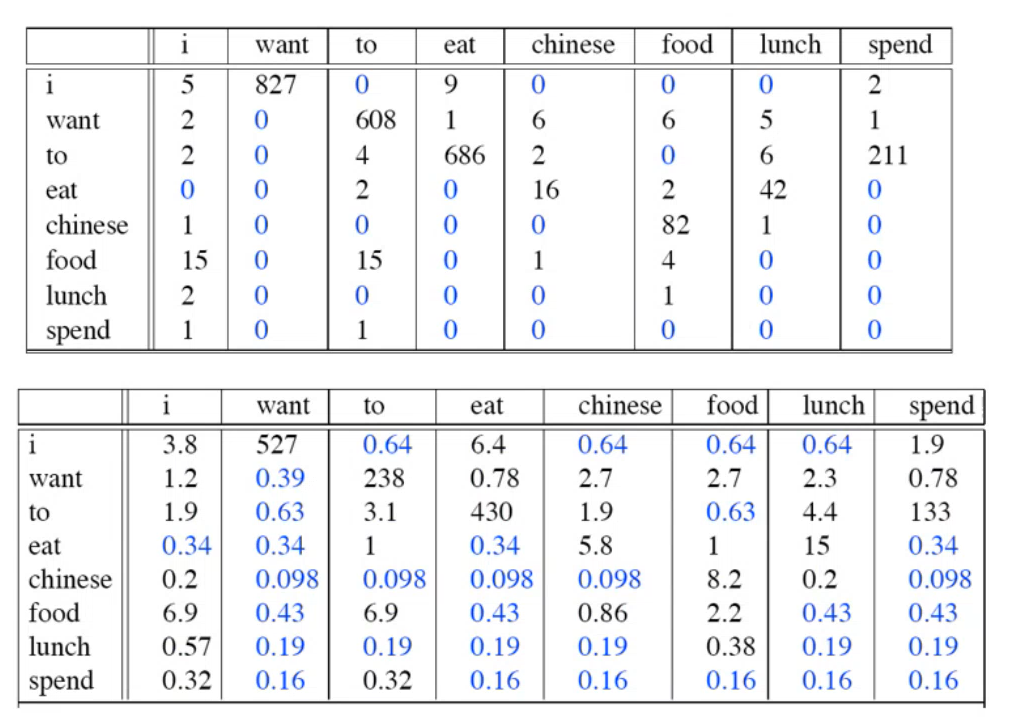
\includegraphics[scale=0.45]{Text Analysis/img/compare.png}
\end{figure}
\\
Ed è dovuto al fattore di discount d:
\begin{center}
    \begin{math}
        d = \frac{c^*}{c} 
    \end{math}
\end{center}
Dove:
\begin{center}
    \begin{math}
        c^* = (c_i+1)\frac{N}{N+V} 
    \end{math}
\end{center}

\newpage

\subsection{Probabilistic Retrieval Models II}
Per fare un search engine che si basa sulla probabilità, noi possiamo usare il concetto di language model. Possiamo andare a guardare in un documento quante volte appare una determinata coppia. 
\\
\begin{figure}[th]
    \centering
    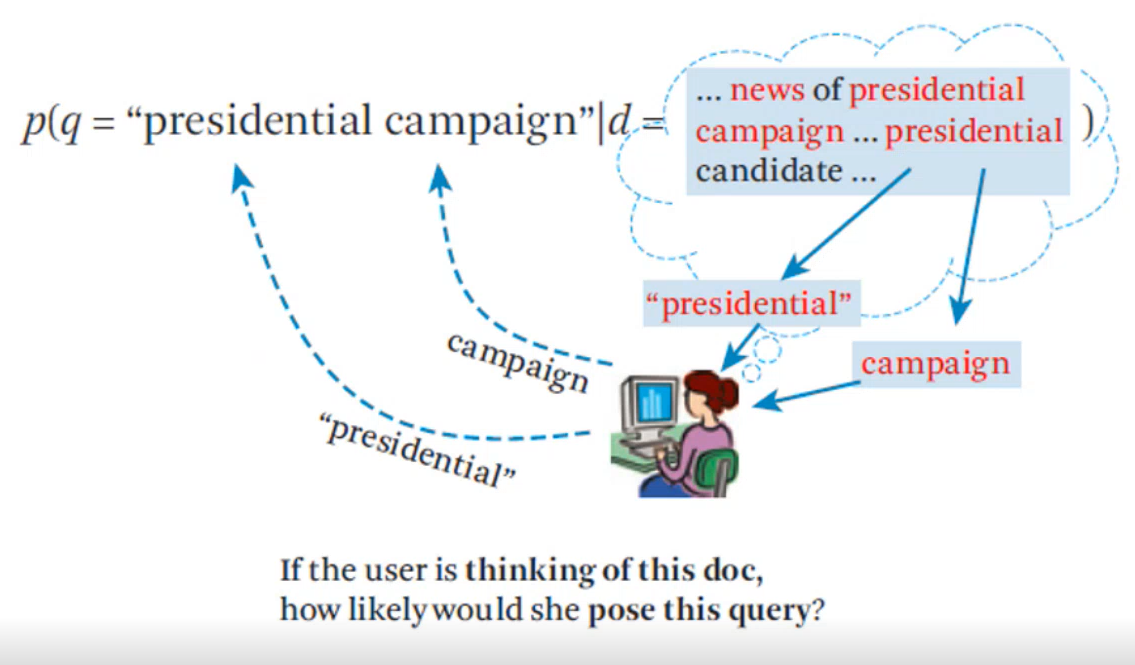
\includegraphics[scale=0.45]{Text Analysis/img/presidentialcampaign.png}
\end{figure}
\\
\textit{Esempio.} Andiamo a guardare nel documento la probabilità che "presidential campaign" sia una domanda per questo specifico documento. Posso usare il language model, e guardare la probabilità delle parole singole all'interno del documento. Se moltiplico tra di loro le due probabilità ottengo la probabilità che la persona stia cercando queste keyword ma che loro non siano necessariamente correlate. \textbf{Assumiamo che la query sia generata campionando parole dal documento.} Ma nella pratica noi abbiamo delle parole correlate!

\subsubsection{The Query Likelihood Retrieval Model}
In un sistema probabilistico, la funzione f(q,d) query-document è data dalla probabilità della query dato il documento \textit{log}p(q$|$d) che posso suddividere sulle parole:
\begin{center}
    \begin{math}
        \sum logp(w_i | d) = \sum c(w,q) logp(w|d)
    \end{math}
\end{center}
Dove il termine c è la frequenza della parola nella query. Quanto è importante quella query q per il documento d? Lo andiamo a calcolare dalla rilevanza, vista per i vector space model. Si calcola come la frequenza della parola nella query (c) per la probabilità della parola nel documento.
\\
Questo modello ha una debolezza: spieghiamo bene con un esempio. La formula funziona bene per ciò che appare sia nel documento che nella query, oppure per quando non appare nella query (che fa 0). Tuttavia, se nella query la parola è presente, mentre nel documento è presente in parte, fa tutto 0, mentre noi vorremmo comunque far finire quel documento nel ranking.
\\
\textit{Esempio.} Parola: Francesco Guerra. Francesco non compare mai, nel documento attuale, ma Guerra sì! Ottiene comunque uno 0.
\\
Dobbiamo quindi trovare una funzione di probabilità che non sia mai 0 quando il valore non è presente. 
\\
\begin{figure}[th]
    \centering
    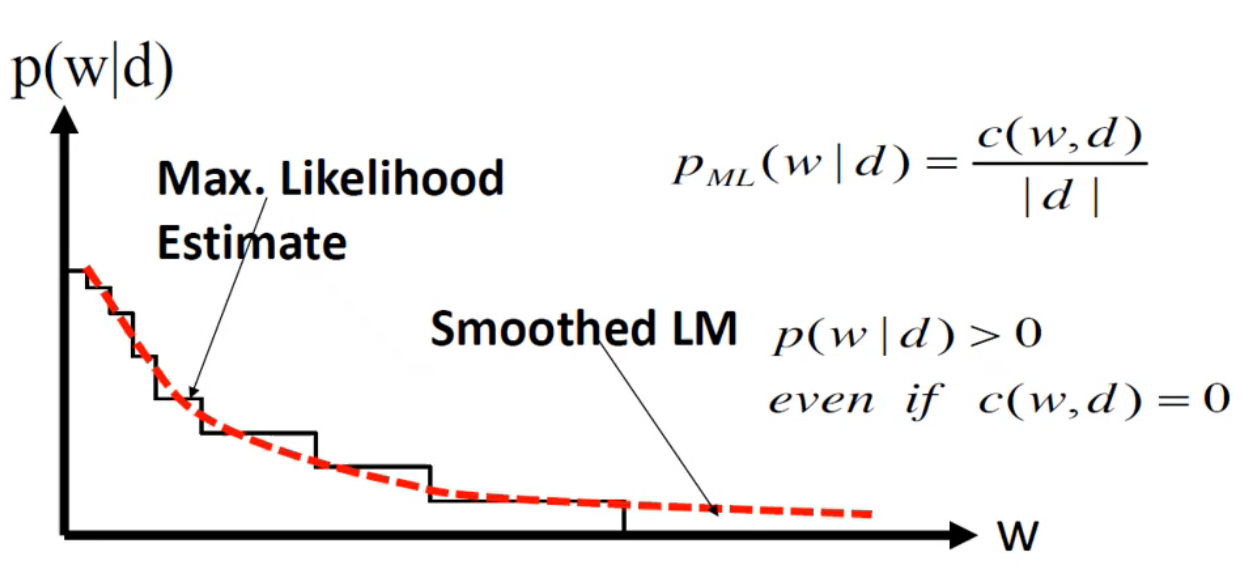
\includegraphics[scale=0.35]{Text Analysis/img/likelihood.png}
\end{figure}

\newpage

\subsubsection{Smoothing della probabilità}
Quale probabilità assegno a quelle parole che attualmente avrebbero 0? Potremmo mettere la probabilità della parola in una generica collection language model, moltiplicata per un $\alpha$ costante. 
\\
\begin{figure}[th]
    \centering
    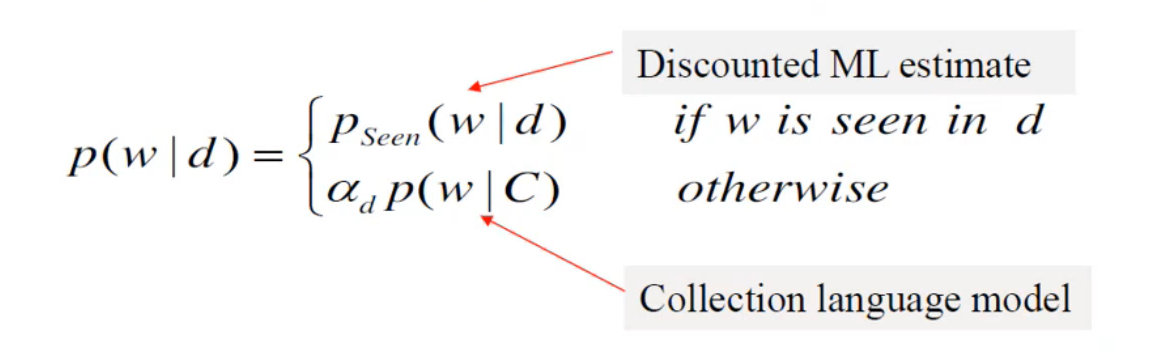
\includegraphics[scale=0.35]{Text Analysis/img/probabo.png}
\end{figure}
\\
Ora riscrivendo la funzione di ranking otteniamo: 
\begin{center}
    \begin{math}
        \sum c(w,q) log \frac{p_{seen}(w|d)}{\alpha_dp(w|C)}+|q|log\alpha_d + \sum c(w,q) logp(w|C)
    \end{math}
\end{center}
Dove mettiamo in mostra tutte le possibili parole, seen e unseen. Quelle che vedi nella formula, sono queste parti, nello specifico:
\\
\begin{figure}[th]
    \centering
    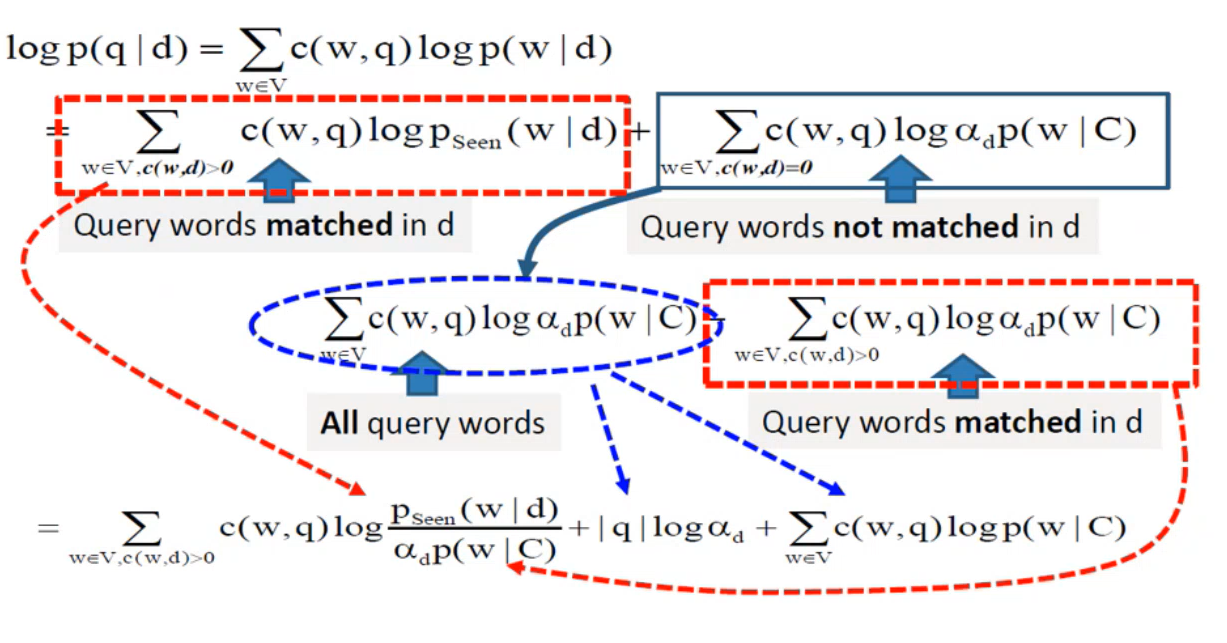
\includegraphics[scale=0.4]{Text Analysis/img/analysis.png}
\end{figure}
\\
Questa è una formula dove abbiamo tutti i componenti della vector space. Al numeratore del primo logaritmo abbiamo la Term Frequency e al denominatore la Document Frequency. L'ultimo termine dell'equazione è ignorabile per il ranking.  

\newpage

\subsection{Search Engine Implementation}
Un sistema IR è composto da 4 componenti: 
\begin{itemize}
    \item \textbf{Tokenizer:} genera l'input del sistema
    \item \textbf{Indexer:} indexing di molti documenti in uno spazio ridotto
    \item \textbf{Scorer/Ranker:} fare lo score dei documenti
    \item \textbf{Learner:} utile quando è presente un feedback
\end{itemize}

\subsubsection{Tokenizer e Indexer} 
Il Tokenizer ha come obiettivo quello di estrarre delle features dal documento; l'Indexer invece mi trova la feature nei documenti sfruttando il concetto di inverted index: un indice che data una parola, mi trova i documenti che contengono quella parola. Normalmente gli inverted index si compongono di due file: 
\begin{itemize}
    \item lexicon, che contiene una lista di parole, quelle contenute nel documento
    \item posting, che contiene i dettagli delle parole
\end{itemize}
\textbf{Come funziona un inverted index?} Si va nei documenti e col tokenizer, si estraggono le parole o i token che riteniamo opportuni. 
\\
\begin{figure}[th]
    \centering
    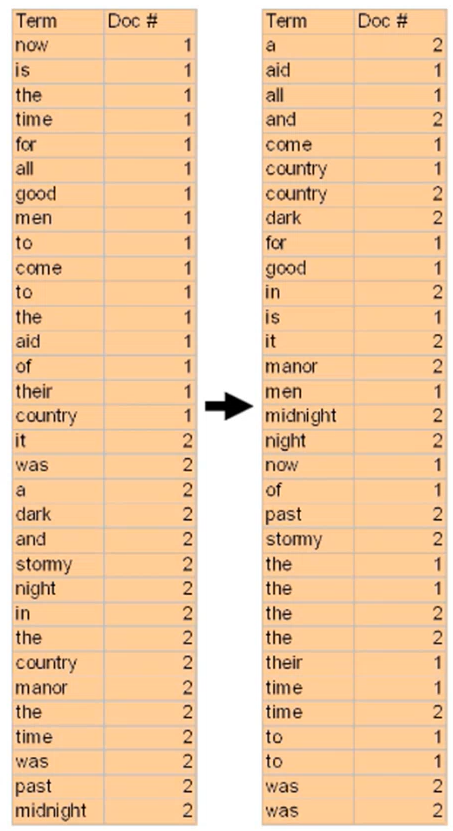
\includegraphics[scale=0.5]{Text Analysis/img/tokenizer.png}
\end{figure}
\\
Un file così è poco utile e confuso. L'indexer fa un orientamento alfabetico e questo è già un esempio di come lavora l'inverted index. L'inverted index può essere infatti diviso in un dictionary che fitta in memoria e contiene termini unici e un file posting che contiene le posizioni dei token, dove sono nel documento (a volte), e viene salvato in memoria. 

\subsubsection{Scorer e Learner}
Data una keyword dobbiamo calcolarne lo score, procedimento svolto dallo scorer sulla base delle informazioni ottenute da tokenizer e indexer, che salverà gli score, facendo poi il sorting dei documenti per rank. 
\\
Il learner usa una cronologia, delle informazioni precedenti per migliorare il risultato. 
\\
\begin{figure}[th]
    \centering
    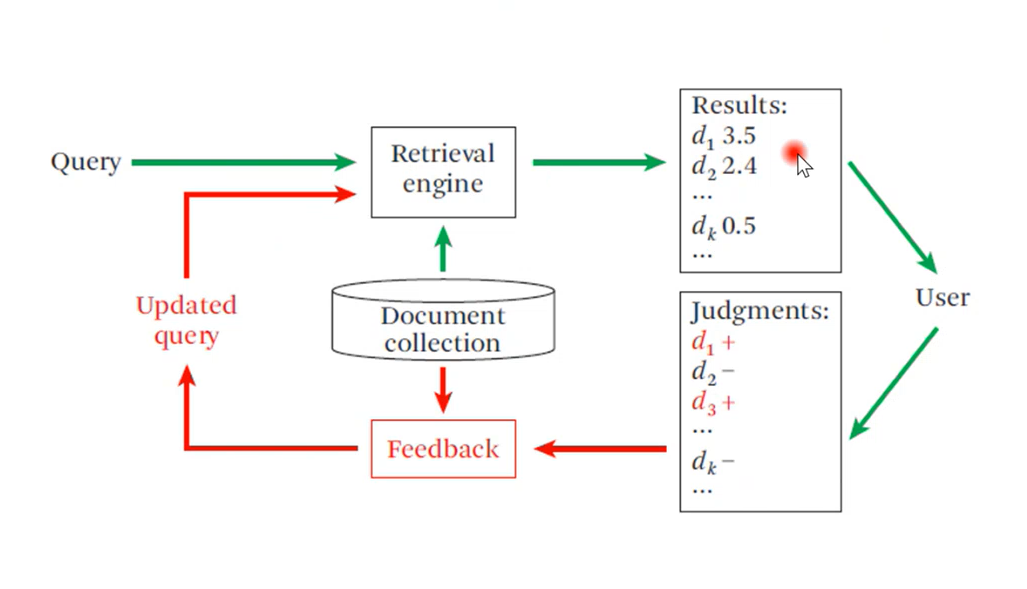
\includegraphics[scale=0.4]{Text Analysis/img/learner.png}
\end{figure}
\\
Il feedback che otteniamo è molto importante. Lo utilizziamo per modificare l'effettiva query dell'utente. Sappiamo che la query q, porta dei determinati documenti per cui noi abbiamo candiato delle query Q, allora modifichiamo la query dell'utente. Faccio un'interrogazione falsa sulla base delle sue richieste passate. 

\subsubsection{Rocchio Feedback}
\begin{figure}[th]
    \centering
    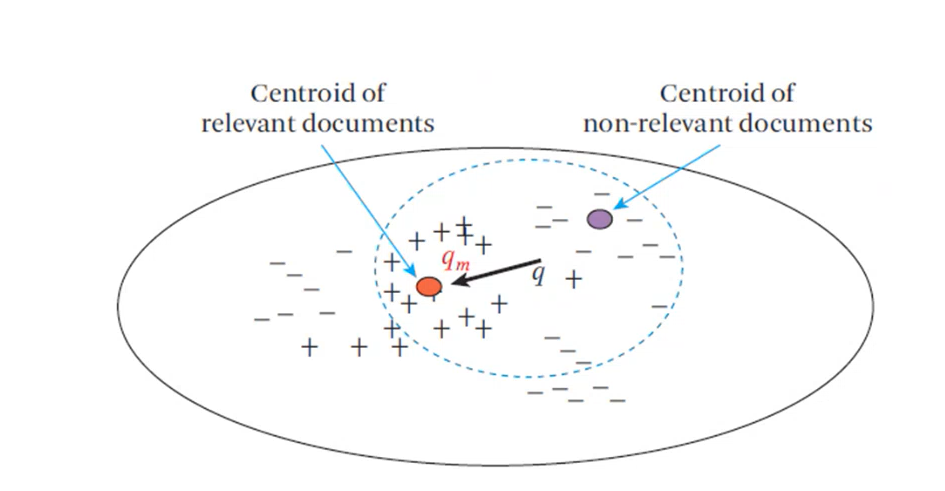
\includegraphics[scale=0.4]{Text Analysis/img/rocchio.png}
\end{figure}
Avvicina la query ad un insieme di documenti rilevanti. Quello che dice il feedback di Rocchio è che: 
\begin{center}
    \begin{math}
        q_m = \alpha \cdot  q + \frac{\beta}{|D_r|} \cdot  \sum d_j - \frac{\gamma}{|D_n|} \cdot  \sum d_j
    \end{math}
\end{center}
Dove gli elementi beta e gamma sono dei coefficienti per i documenti rilevanti e quelli useless. q è il vettore della query originale, Dr e Dn sono relevant e non-relevant documents, mentre i parametri aggiunti servono per calibrare il movimento del vettore originale. 
\\
I coefficienti sono molto delicati: ad esempio, se $\alpha$ fosse 0, ci si baserebbe molto solo su il passato di q, quindi overfitterremmo sulla query dell'utente. Nella pratica, andremo incontro ad un particolare problema: performeremmo un calcolo molto costoso, per aggiornare pesi e centroidi. I non-relevant, per di più non saranno per niente utili e dovremo fare attenzione alla questione overfitting (i parametri devono essere ricavati empiricamente).

\newpage

\subsection{Text classification}
Consiste nel:
\begin{itemize}
    \item Assegnare generi, categorie\dots
    \item Spam detection
    \item Identificazione
\end{itemize}
E molte altre cose. Quindi quello che si può fare è dato un documento d, e un set di classi Y, predire una classe $y_i$ per d. Si può fare con delle regole, oppure esistono anche delle tecniche che si basano su Machine Learning. 
\\
\textbf{Attenzione!} Le tecniche di machine learning funzionano perfettamente, ma vanno in crisi: ad esempio, nella sentiment analysis. Immaginiamo la frase:
\begin{center}
    Marco è bello
\end{center}
Che ha accezione positiva. Ma basta aggiungere una parola:
\begin{center}
    Marco non è bello
\end{center}
Per cambiarne completamente il significato. E per un algoritmo di ML, capire questo è complesso. 

\subsubsection{Computational Lexical Semantics}
Lavorare con la semantica delle parole, assegnargli un significato. Le macchine non sanno il significato delle parole. Ad esempio, trovare le relazioni tra parole, trovare le similitudini, anche trovare un modo per disambiguare una parola (ho 20 anni, venti sarebbe anche plurale di vento).
\\
\textbf{Cosa fai quando non sai il significato di una parola?} Guardi sul vocabolario. Ma c'è un problema: sul vocabolario, ci sono i cosiddetti \textit{lemmi}. Un lemma è ad esempio: io mangio, il suo lemma è mangiare sul vocabolario e come puoi vedere sono estremamente diversi. Quando si parla di parole correlate, potremmo dire ad esempio caffè e tazza. Oppure una relazione tassonomica, dal più grande al più piccolo, \textit{villetta} è sottoinsieme di casa (esempio di tassonomia). In particolare si dice \textbf{iponimia} se ci si muove verso il basso e \textbf{ipernimia} se ci si muove verso l'alto. Ma il vocabolario questo tipo di informazioni non le contiene quindi anche usarlo è qualcosa di riduttivo. 
\\
Usare un vocabolario è una cosa complessa per una macchina. \textit{Esempio.} Definizione di rosso:
\begin{center}
    Colore del sangue, o di un rubino.
\end{center}
La definizione di sangue invece è:
\begin{center}
    Il liquido rosso che circola nelle vene, arterie e cuore degli animali.
\end{center}
Le due definizioni di facile interpretazione per un umano, meno facile per una macchina che nota il collegamento ma non sa come utilizzarlo. WordNet è stato il primo dizionario lessicale, utile per applicazioni, fatto apposta per codificare un vocabolario utilizzabile da una macchina. 

\newpage

Per la disambiguation, esistono dei dataset appositi che possono essere utilizzati in ML con un approccio \textit{supervised}. Per fare disambiguazione, esiste l'algoritmo di Lesk, che confronta un termine con il suo significato su WordNet e insieme al contesto riesce a disambiguare:
\\
\begin{figure}[th]
    \centering
    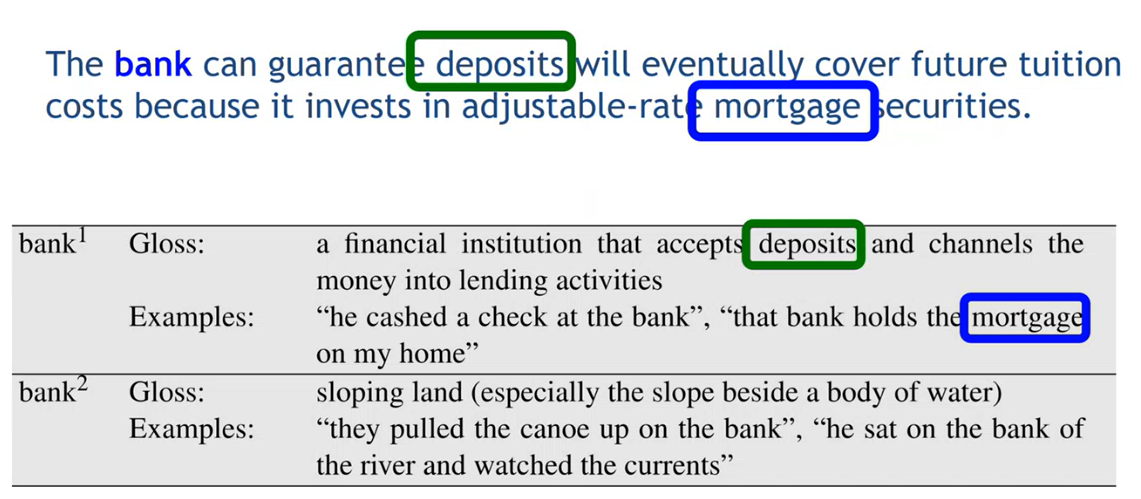
\includegraphics[scale=0.4]{Text Analysis/img/Lesk.png}
\end{figure}
\\
Come si può vedere dall'esempio nell'immagine, l'algoritmo di Lesk trova dei match nella definizione di baca come istituzione, e non come banco. 

\subsubsection{Vector semantics and embeddings}
Possiamo pensare di avere parole simili, in \textbf{contesti} simili. Non ci serve necessariamente un vocabolario per capire delle parole ma basta il contesto. 
\begin{center}
    \textit{A bottle of tesguino.}
    \\
    \textit{Everybody like tesguino.}
    \\
    \textit{Tesguino makes you drunk.}
    \\
    \textit{We make tesguino out of corn.}
\end{center}
Da queste frasi riusciamo perfettamente a capire cosa sia il tesguino, semplicemente dal contesto! (O almeno, lo immaginiamo)
\\
Iniziamo a vedere un approccio per cui rappresentiamo le parole come un vettore e questo vettore rappresenta il significato che attribuiamo a tale parola. Per costruirli sfruttiamo la \textbf{distributional hypothesis} che semplicemente sostiene che le parole vicine siano in un qualche modo correlate. Attraverso gli embeddings poi possiamo raggruppare e fare dei clusters con parole dal signidicato simile. 
\\
Possiamo costruire quattro tipologie di vettori:
\begin{itemize}
    \item sparse vector representations
    \item SVD (singular value decomposition) and LSA (Latent Semantic Analysis)
    \item neural networks models
    \item contextualized embeddings
\end{itemize}

\newpage

\subsubsection{Sparse vector representations: Term-document matrix}
Ogni riga rappresenta una parola nel vocabolario e ogni colonna rappresenta un documento di una collection. 
\\
\begin{figure}[th]
    \centering
    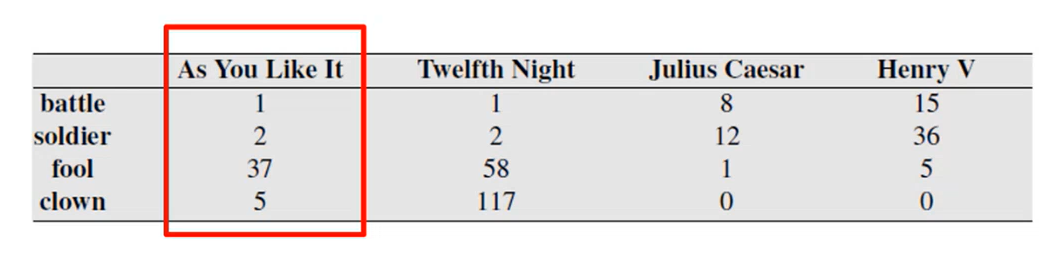
\includegraphics[scale=0.5]{Text Analysis/img/termdocument.png}
\end{figure}
\\
L'embedding lo costruisco su questa matrice: battle, sarà un vettore 1,1,8,15. Quello che facciamo quindi è creare una matrice di frequenza. 

\subsubsection{Sparse vector representations: word-word or term-context matrix}
Sulle righe e sulle colonne abbiamo delle parole: il numero rappresenta se le parole compaiono insieme. Contiamo le 3 parole prima e le 3 dopo e vediamo il risultato del conteggio. Poi dipende quante parole vogliamo guardare, possiamo arrivare anche alle 10 parole ma ricerchiamo molto il significato. 
\\
\begin{figure}[th]
    \centering
    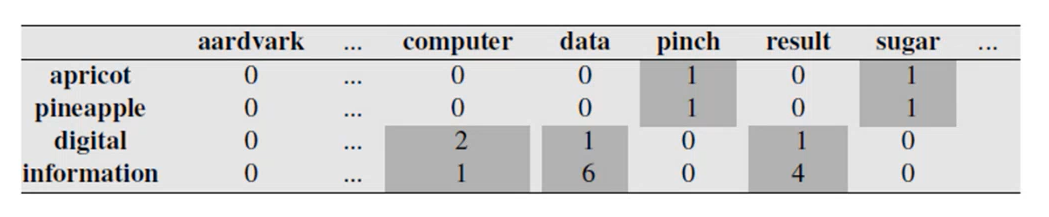
\includegraphics[scale=0.5]{Text Analysis/img/wordword.png}
\end{figure}
\\
Però queste matrici sono molto grandi.

\subsubsection{Positive Pointwise Mutual Information}
\begin{center}
    \begin{math}
        PPMI(w,c) = max(log_2 \frac{P(w,c)}{P(w) P(c)}, 0)
    \end{math}
\end{center}
Molto spesso, viene negativa quando il contesto non c'entra nulla con la parola. Si usa la positive per arrotondare a 0. 

\newpage

\subsubsection{Singular Value Decomposition (SVD) e Latent Semantic Analysis (LSA)}
Prende una distribuzione di valori, e ruota lungo gli assi per trovare una dimensionalità inferiore senza perdere informazione. 
\begin{center}
    \begin{math}
        A_{[m \times n]} = U_{[m \times r]} \Sigma_{[r \times r]} (V_{[n \times r]})^T
    \end{math}
\end{center}
Dove A è la matrice di input, U sono i left singular vector e V sono i right singular vectors, sigma sono i singular values. m sono i documents, n i terms, e r sono i concepts. Sigma è una matrice diagonale di valori ordinati in ordine decrescente. 
\\
\begin{figure}[th]
    \centering
    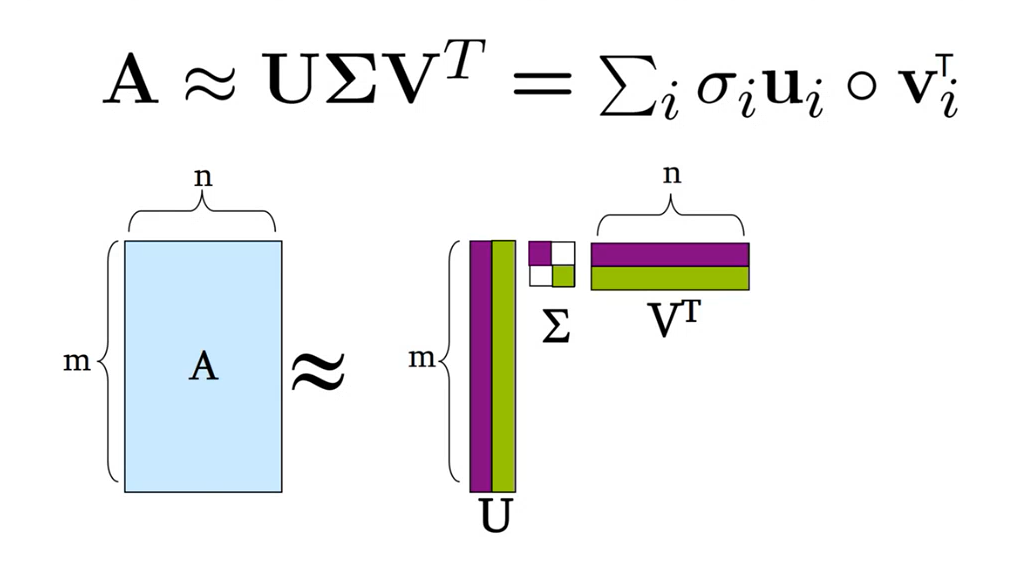
\includegraphics[scale=0.4]{Text Analysis/img/svd.png}
\end{figure}
\\
Quello che fa è costruire una matrice densa, partendo da una sparsa. Elimino degli elementi da un certo punto in poi. Cosa succede? Che ho un'approssimazione della matrice originale, ma nel ML non è un male approssimare, generalizzo di più. Come decido però che approssimazione fare? Siamo nel caso di LSA (Latent Semantic Analysis) chiamata anche TruncatedSVD se manteniamo almeno un 80-90\% dell'energia. 

\subsubsection{Word2vec}
Attraverso questa tecnica creiamo dei vettori per ogni parola con le parole vicine ad essa in questo momento. Diventa un problema di classificazione binaria. Sistema rivoluzionario poichè self-supervised, coglie da solo le relazioni tra parole senza necessità di label. 
\\
Gli embeddings creati con questo metodo sono statici, impara un singolo embedding per ogni parola. Esistono tecniche più avanzate più recenti che guardano bene anche al contesto. La versione skip-gram:
\begin{enumerate}
    \item Tratta la parola e quella vicina come esempi positivi
    \item Prende delle parole casuali dal lexicon come esempi falsi
    \item Usa la logistic regression per classificare esempi buoni e negativi
    \item Usa i pesi della regressione come embeddings
\end{enumerate}
Skip-gram usa due embeddings per ogni parola, uno per una parola come target e uno per quando diventa contesto per altre parole, e il risultato è la somma dei due.
\\
Le parole positive sono facili da selezionare (sono quelle vicine a quella target) quelle negative vengono selezionate in base alla loro probabilità nel documento e quante sceglierne è un iperparametro. Normalmente si mette la weighted unigram frequency, è una probabilità pesata non quella pura, gestita tramite un parametro anch'essa. Questo perchè per la probabilità di Zipf, ci sarebbero poche parole tanto frequenti e molte parole poco frequenti. Con il parametro andiamo a schiacciare quelle tanto frequenti, mentre gonfiamo quelle poco frequenti. 
\\
\textbf{Importante.} Gli embeddings godono di una particolare regola: la distanza calcolata tra due parole di senso diverso, ma semanticamente collegate (ad esempio Re e Regina) e delle parole a loro correlate (ad esempio Uomo e Donna) è uguale. Quindi la distanza che c'è tra re e uomo è uguale a quella che c'è tra regina e donna. Questa proprietà prende il nome di \textit{parallelogramma}.

\subsection{Neural Networks Basics}
Grazie a questi potenti algoritmi non abbiamo problemi degli altri algoritmi ML. Essi rientrano nella categoria DL (Deep Learning) e sono completamente blackbox. Essi si basano sul concetto di neurone, che è fatto come un neurone umano:
\begin{itemize}
    \item ha un input, che è l'informazione dal neurone nel layer precedente o l'input di sistema
    \item ha una funzione di attivazione, che costruisce il valore di output 
    \item ha un output che viene passato al layer successivo, o all'uscita dell'algoritmo
\end{itemize}
Esistono diverse funzioni di attivazione, la più importante sicuramente è la ReLU (rectified linear unit) che è una funzione = 0 per x negative, poi restituisce x (quindi è una retta). 

\subsubsection{Feed Forward Neural Networks}
Prendono questo nome perchè per scorrerli si va dal primo layer all'ultimo. Esistono altri modi per percorrerli. Si ha un input layer x, una serie di hidden layers h, e un output layer y. Negli hidden layer l'informazione viene elaborata e esce dagli output, dove per una interrogazione vengono fuori più risposte con un relativo score dato dalla funzione softmax che normalizza a 1 in modo da rendere gli score capibili anche da un umano. 
\\
\textbf{Ma come la alleno su una frase?} Potrei prendere gli embeddings, e farne la media, o prendere il valore max o min. Possiamo oppure unirli tutti: questa operazione prende il nome di pooling. 
\\
\begin{figure}[th]
    \centering
    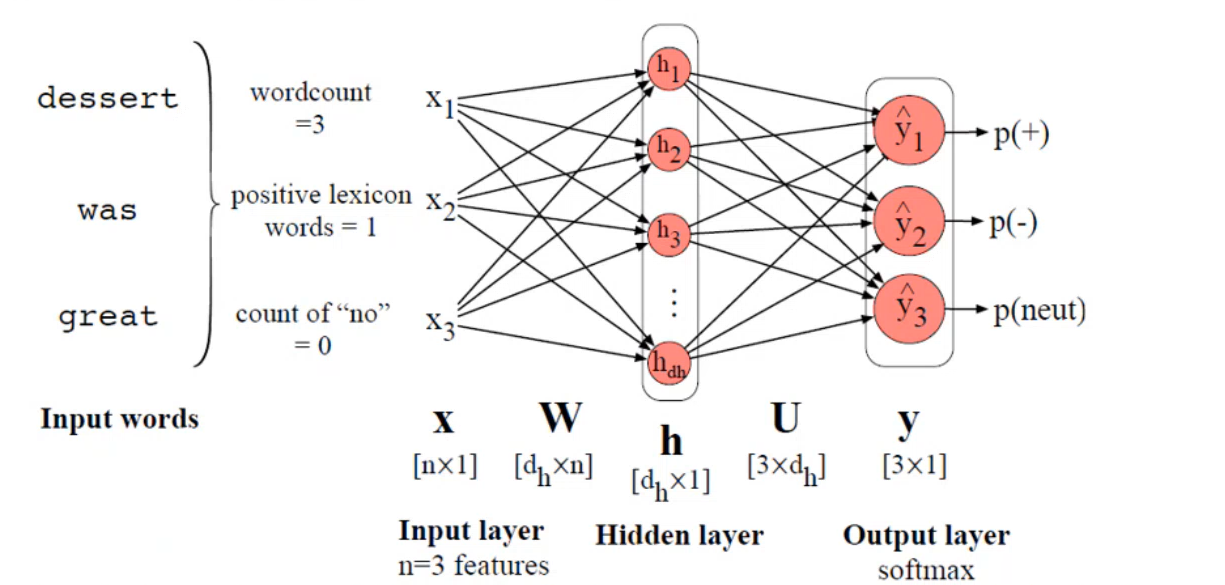
\includegraphics[scale=0.5]{Text Analysis/img/NNforNLP.png}
\end{figure}

\newpage

\subsection{Recurrent Neural Networks}
Sono particolari reti neurali che considerano la risposta precedente, e vengono utilizzate in NLP per l'analisi del testo. Tiene conto della posizione delle parole, la sequenza viene rispettata. 
\\
Ha degli svantaggi: necessita di tanti dati e perde efficacia con testi lunghi, non rilevando le relazioni tra parole distanti. Come possono due paroli distanti avere una correlazione? Ad esempio, i pronomi riferiti al soggetto esplicito della frase. 

\subsubsection{Sequence classification}
Metodo di funzionamento per la text classification con Recurrent NN. Abbiamo come input una frase e come risultato ottengo una prediction e un hidden layer che conosce tutte le parole. Possiamo quindi sfruttare quell'H per fare classificazione su altre frasi. Proprio in questo sta il suo vantaggio: poter allenare H e riutilizzarlo.
\\
Ogni neurone ha una doppia funzione che è classificare e fornire contesto per la parola successiva. Difficile mantenere buone prestazioni. Esiste anche l'architettura LSTM (Long-Short Term Memory) che viene utilizzata in questo ambito, e aggiunge all'architettura base delle RNN un \textit{forget:} decide gli elementi da salvare e quali possono essere dimenticati, attraverso una sigmoide finale che decide gli elementi da dimenticare. 

\subsection{Contextualized embeddings}
Mentre nel word2vec viene fatto un embedding per ogni parola, in questo caso gli embeddings cambiano in base al contesto: state of art è il meccanismo di attenzione dei transformers. 

\subsubsection{Transformers}
Architettura particolare che si basa sul meccanismo di attenzione: il contesto delle parole è variabile e dipendente dalla frase. Viene realizzato attraverso una rete encoder-decoder e possiamo ottenere un risultato di questo tipo:
\\
\begin{figure}[th]
    \centering
    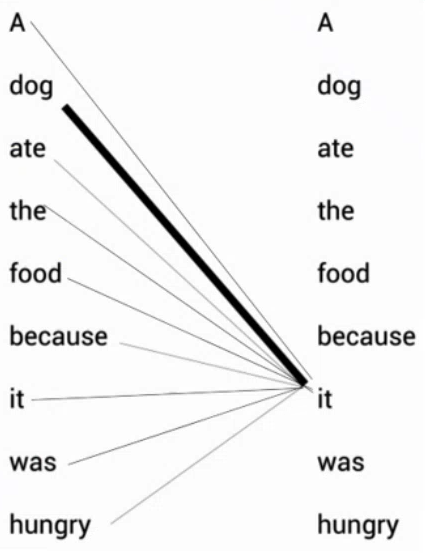
\includegraphics[scale=0.5]{Text Analysis/img/selfattention.png}
\end{figure}
\\
Ovvero la parola it guadagna il significato di dog, vengono correlate. Questo tipo di meccanismo serve principalmente per frasi molto lunghe. Sfrutta la conoscenza delle parole future, che non è scontato sapere. 
\\
\textbf{Ma come funziona il meccanismo di self-attention?} Il calcolo dei confronti nella matrice ha come risultato uno score per ogni valore della query e ogni key, anche quelle che si seguono. Per evitarlo, vengono azzerate, in modo da eliminare ogni tipo di conoscenza sulle loro relazioni. L'attenzione è quadratica quindi va monitorata poichè troppo costosa. L'input viene usato in modo aggiuntivo: sommiamo i valori dell'input per non perdere informazione (\textit{residual block}).

\subsubsection{Multihead attention mechanism}
Lo stesso input viene processato da n blocchi transformer, ogni head produce un risultato per lo stesso input, ogni blocco è chiamato head. In questa architettura viene sfruttato anche il concetto di positional encoding, per fornire informazioni utili sulla posizione dell'input (sapere la posizione di una parola all'interno della frase). 
\\
\begin{figure}[th]
    \centering
    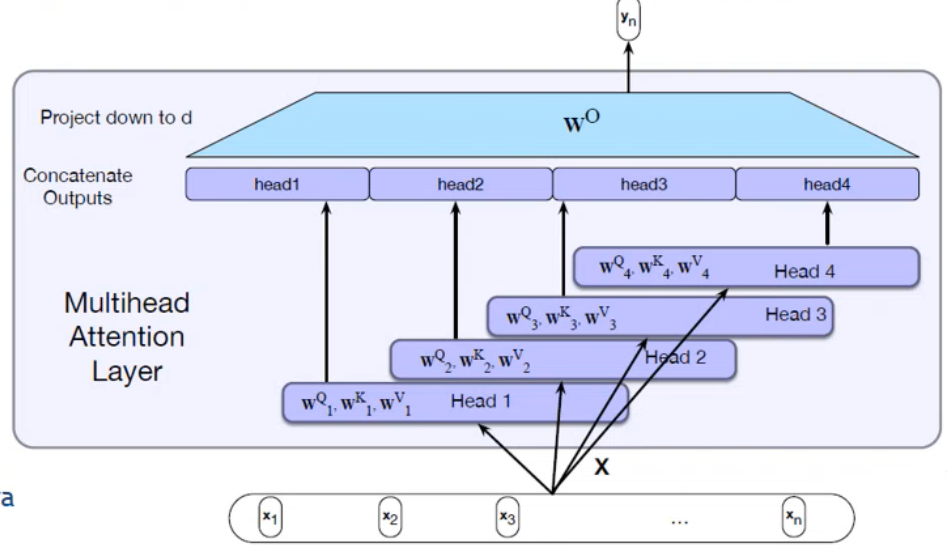
\includegraphics[scale=0.5]{Text Analysis/img/multihead.png}
\end{figure}
\\